\experiment{Circular Queue}{11/10/2023}

\section{Aim}
Write a menu driven C Program to implement a circular queue using arrays with the
following operations:
\\a. Insert an element to the queue.
\\b. Delete an element from the queue.
\\c. Display the contents of the queue after each operation.

\section{Algorithm}
 {\fontfamily{lmtt}\selectfont

  \subsection{Create Circular Queue}
  \begin{enumerate}[label=\arabic*:,left=0pt]
    \item \textbf{Start}
    \item Define a structure for a queue:
          \begin{enumerate}[label=2.\arabic*.]
            \item Include \texttt{front}, \texttt{back}, \texttt{size}, and an integer array \texttt{arr[100]}.
          \end{enumerate}
    \item Create a function \texttt{createQueue()}:
          \begin{enumerate}[label=3.\arabic*.]
            \item Allocate memory for a new queue \texttt{q}.
            \item Set \texttt{q->front} and \texttt{q->back} to -1, and \texttt{q->size} to 5.
          \end{enumerate}
    \item Return \texttt{q}.
    \item \textbf{Stop}
  \end{enumerate}

  \subsection{Enqueue Function}
  Create a function \texttt{enqueue(q, data)}:
  \begin{enumerate}[label=\arabic*:,left=0pt]
    \item \textbf{Start}
    \item If \texttt{q->front} is -1 and \texttt{q->back} is -1:
          \begin{enumerate}[label=2.\arabic*.]
            \item Set \texttt{q->front} and \texttt{q->back} to 0.
            \item Set \texttt{q->arr[q->back]} to \texttt{data}.
            \item Return.
          \end{enumerate}
    \item If \texttt{q->back} is equal to \texttt{q->size - 1}:
          \begin{enumerate}[label=2.\arabic*.]
            \item Check if \texttt{q->front} is greater than 0:
                  \begin{enumerate}[label=3.\arabic*.]
                    \item Set \texttt{q->back} to 0.
                    \item Set \texttt{q->arr[q->back]} to \texttt{data}.
                    \item Return.
                  \end{enumerate}
            \item Otherwise, print "Queue overflow" and return.
          \end{enumerate}
    \item Check if \texttt{q->back + 1} is equal to \texttt{q->front}:
          \begin{enumerate}[label=2.\arabic*.]
            \item Print "Queue overflow" and return.
          \end{enumerate}
    \item Increment \texttt{q->back}.
    \item Set \texttt{q->arr[q->back]} to \texttt{data}.
    \item \textbf{Stop}
  \end{enumerate}

  \subsection{Dequeue Function}
  Create a function \texttt{dequeue(q)}:
  \begin{enumerate}[label=\arabic*:,left=0pt]
    \item \textbf{Start}
    \item Declare \texttt{removed}.
    \item Check if \texttt{q->back} is equal to \texttt{q->front}:
          \begin{enumerate}[label=2.\arabic*.]
            \item Check if \texttt{q->front} is -1:
                  \begin{enumerate}[label=3.\arabic*.]
                    \item Print "Queue underflow" and return.
                  \end{enumerate}
            \item Set \texttt{removed} to \texttt{q->arr[q->front]}.
            \item Set \texttt{q->front} and \texttt{q->back} to -1.
          \end{enumerate}
    \item Else:
          \begin{enumerate}[label=2.\arabic*.]
            \item Set \texttt{removed} to \texttt{q->arr[q->front]}.
            \item Increment \texttt{q->front}.
            \item Set \texttt{q->front} to \texttt{q->front \% q->size}.
          \end{enumerate}
    \item Print "Removed Element =", \texttt{removed}.
    \item \textbf{Stop}
  \end{enumerate}

  \subsection{Display Function}
  Create a function \texttt{display(q)}:
  \begin{enumerate}[label=\arabic*:,left=0pt]
    \item \textbf{Start}
    \item Check if \texttt{q->front} is -1 and \texttt{q->back} is -1:
          \begin{enumerate}[label=2.\arabic*.]
            \item Print "Queue is empty!" and return.
          \end{enumerate}
    \item Print "Queue elements are":
          \begin{enumerate}[label=2.\arabic*.]
            \item If \texttt{q->back} is greater than or equal to \texttt{q->front}:
                  \begin{enumerate}[label=3.\arabic*.]
                    \item Loop from \texttt{q->front} to \texttt{q->back}:
                          \begin{enumerate}[label=4.\arabic*.]
                            \item Print \texttt{q->arr[i]}, followed by a space.
                          \end{enumerate}
                  \end{enumerate}
            \item Otherwise:
                  \begin{enumerate}[label=3.\arabic*.]
                    \item Loop from \texttt{q->front} to \texttt{q->size - 1}:
                          \begin{enumerate}[label=4.\arabic*.]
                            \item Print \texttt{q->arr[i]}, followed by a space.
                          \end{enumerate}
                    \item Loop from 0 to \texttt{q->back}:
                          \begin{enumerate}[label=4.\arabic*.]
                            \item Print \texttt{q->arr[i]}, followed by a space.
                          \end{enumerate}
                  \end{enumerate}
          \end{enumerate}
    \item Print a newline.
    \item \textbf{Stop}
  \end{enumerate}

  \subsection{Main Function}
  In the \texttt{main} function:
  \begin{enumerate}[label=\arabic*:, start=1]
    \item \textbf{Start}
    \item Create a circular queue \texttt{q} using \texttt{createQueue()}.
    \item Initialize \texttt{ch}.
    \item \textbf{Start Menu Loop}
          \begin{enumerate}[label=4.\arabic*:, start=1]
            \item Print menu options.
            \item Take user input for \texttt{ch}.
            \item If \texttt{ch} is 1:
                  \begin{enumerate}[label=4.1.\arabic*:, start=1]
                    \item Take user input for \texttt{x}.
                    \item Call \texttt{enqueue(q, x)}.
                  \end{enumerate}
            \item If \texttt{ch} is 2, call \texttt{dequeue(q)}.
            \item If \texttt{ch} is 3, call \texttt{display(q)}.
            \item If \texttt{ch} is 4, exit the loop.
            \item If \texttt{ch} is none of the above, print "Invalid option!".
          \end{enumerate}
    \item \textbf{Stop Menu Loop}
    \item \textbf{Stop}
  \end{enumerate}

 }
\section{C Program}
\begin{lstlisting}[label={list:c_program:circular_queue}]
#include <stdlib.h>
#include <stdio.h>

typedef struct queue
{
  int front;
  int back;
  int size;
  int arr[100];
} queue;

queue *createQueue();
void enqueue(queue *q, int data);
void dequeue(queue *q);
void display(queue *q);

int main()
{
  queue *q = createQueue();
  int ch;
  printf("1)Enqueue\n2)Dequeue\n3)Display\n4)Exit\n");
  do
  {
    printf("Choice: ");
    scanf("%d", &ch);
    if (ch == 1)
    {
      int x;
      printf("\nEnter the data: ");
      scanf("%d", &x);
      printf("\n");
      enqueue(q, x);
    }
    else if (ch == 2)
    {
      dequeue(q);
    }
    else if (ch == 3)
    {
      display(q);
    }
    else if (ch != 4)
    {
      printf("\nInvalid option!\n");
    }
  } while (ch != 4);
}

queue *createQueue()
{
  queue *q = (queue *)malloc(sizeof(queue));
  q->front = -1;
  q->back = -1;
  q->size = 5;
  return q;
}

void enqueue(queue *q, int data)
{
  if (q->front == -1 && q->back == -1)
  {
    q->front = 0;
    q->back = 0;
    q->arr[q->back] = data;
    return;
  }
  else if (q->back == q->size - 1)
  {
    if (q->front > 0)
    {
      q->back = 0;
      q->arr[q->back] = data;
      return;
    }
    else
    {
      printf("\nQueue overflow!\n");
      return;
    }
  }
  else if (q->back + 1 == q->front)
  {
    printf("\nQueue overflow!\n");
    return;
  }
  q->back++;
  q->arr[q->back] = data;
}

void dequeue(queue *q)
{
  int removed;
  if (q->back == q->front)
  {
    if (q->front == -1)
    {
      printf("\nQueue underflow!\n");
      return;
    }
    removed = q->arr[q->front];
    q->front = -1;
    q->back = -1;
  }
  else
  {
    removed = q->arr[q->front];
    q->front++;
    q->front %= q->size;
  }
  printf("\nRemoved Element = %d\n", removed);
}

void display(queue *q)
{
  if (q->front == -1 && q->back == -1)
  {
    printf("\nQueue is empty!\n");
    return;
  }
  printf("\nQueue elements are\n");
  if (q->back >= q->front)
  {
    for (int i = q->front; i <= q->back; i++)
    {
      printf("%d ", q->arr[i]);
    }
  }
  else
  {
    for (int i = q->front; i < q->size; i++)
    {
      printf("%d ", q->arr[i]);
    }
    for (int i = 0; i <= q->back; i++)
    {
      printf("%d ", q->arr[i]);
    }
  }
  printf("\n");
}

\end{lstlisting}

\section{Output}
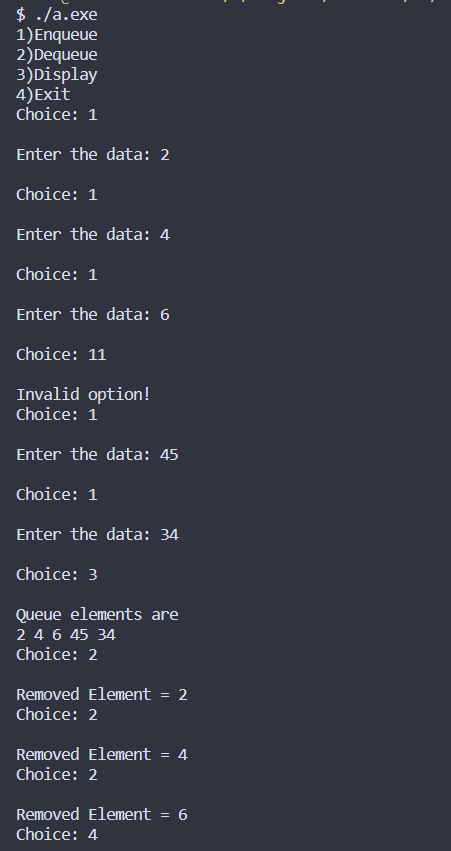
\includegraphics[]{Cycle_1/Outputs/CircularQueue.png}
\section{Result}
Circular queue implemented using arrays. The program was executed and output verified.